\section{Esercizio 2 -- Sistema ROM + M}
\subsection{Esercizio 2.1}
Per la risoluzione dell'esercizio è stata adottata un'architettura modulare [Figura \ref{fig:2_1_ROM_M}]. Si sono utilizzati due componenti principali: la memoria ROM e la macchina M, che esegue la trasformazione sugli 8 bit in ingresso per restituire 4 bit in uscita. Entrambi i componenti sono dichiarati come entità separate con relativi port e generici che consentono flessibilità nella configurazione. La memoria ROM è implementata come un array di 16 locazioni, ognuna contenente un valore a 8 bit. L'indirizzo fornito al sistema determina quale locazione della memoria viene selezionata, e il valore corrispondente viene quindi inviato alla macchina combinatoria. La macchina a sua volta restituisce un risultato a 4 bit.

\begin{figure}[h]
    \centering
    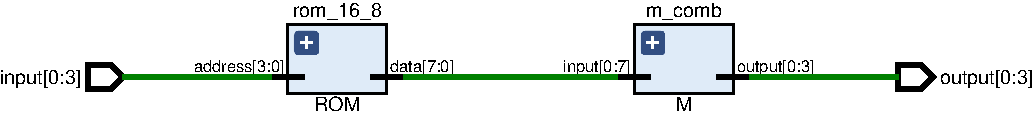
\includegraphics[width=0.8\linewidth]{img/2_1_ROM_M.pdf}
    \caption{Schema dell'architettura ROM + M}
    \label{fig:2_1_ROM_M}
\end{figure}

\subsubsection{Implementazione}
La soluzione proposta implementa un sistema composto da una memoria ROM di 16 locazioni da 8 bit ciascuna e una macchina combinatoria M. La memoria ROM è progettata per essere puramente combinatoria, e la macchina combinatoria prende in ingresso 8 bit e restituisce 4 bit in base al valore del bit meno significativo dell'ingresso. 

Prima di analizzare il sistema complessivo poniamo attenziona sull’implementazione degli altri due componenti ovvero la ROM e la macchina.

\paragraph{Memoria ROM.} Essa è composta da 16 locazioni, ognuna contenente un valore di 8 bit. 

\begin{code}
    \inputminted{vhdl}{vhdl/2_ROM.vhd}
    \caption{Implementazione della memoria ROM}
    \label{cod:2_ROM}
\end{code}

L'entity è la parte del codice che descrive i segnali di ingresso e uscita del componente ROM.

\begin{itemize}
    \item \texttt{address}: è un segnale di ingresso di 4 bit (\texttt{std\_logic\_vector(3 downto 0)}). Poiché ha 4 bit, può assumere 16 valori diversi.
    \item \texttt{data}: è un'uscita di 8 bit (\texttt{std\_logic\_vector(7 downto 0)}) che contiene il valore memorizzato all'indirizzo richiesto.
\end{itemize}

L'architettura, che è \texttt{behavioral} [Codice sorgente \ref{cod:2_ROM}], è la parte in cui viene definito il comportamento interno della ROM. Qui viene utilizzato un array inizializzato di 16 elementi (\texttt{rom\_16\_8}), ognuno dei quali è un vettore di 8 bit (\texttt{std\_logic\_vector(7 downto 0)}). 

Questi elementi rappresentano i dati che la ROM restituirà in base all'indirizzo in ingresso. L'attributo \texttt{rom\_style} con valore \texttt{block} indica che questa ROM deve essere implementata come una ``block RAM" all'interno di una FPGA, ottimizzando l'uso delle risorse hardware.

Il processo \texttt{process(address)} viene eseguito ogni volta che varia il valore di \texttt{address}.

La riga \texttt{data <= ROM(to\_integer(unsigned(address)))} fa il seguente lavoro:
\begin{enumerate}
    \item Converte \texttt{address} (che è un \texttt{std\_logic\_vector}) in un numero intero, interpretandolo come intero senza segno (\texttt{to\_integer(unsigned(address))}).
    \item Usa questo valore intero come indice per accedere alla tabella ROM e restituisce il valore corrispondente in \texttt{data}.
\end{enumerate}

\paragraph{Macchina M.} Un circuito combinatorio che prende in ingresso un vettore di 8 bit e produce in uscita un vettore di 4 bit. Il funzionamento del circuito è piuttosto semplice: l'uscita viene generata applicando l'operazione logica AND su coppie di bit dell'ingresso.

\begin{code}
    \inputminted{vhdl}{vhdl/2_M.vhd}
    \caption{Implementazione della macchina M}
    \label{cod:2_M}
\end{code}

L'entity è la parte del codice che descrive i segnali di ingresso e uscita della macchina M.

\begin{itemize}
    \item \texttt{input}: è un vettore di 8 bit (\texttt{std\_logic\_vector(0 to 7)}), quindi può contenere 256 combinazioni diverse di 0 e 1.
    \item \texttt{output}: è un vettore di 4 bit (\texttt{std\_logic\_vector(0 to 3)}) e rappresenta il risultato delle operazioni logiche effettuate sui bit dell'input.
\end{itemize}

L’architettura, che è \texttt{dataflow} [Codice sorgente \ref{cod:2_M}], è la parte in cui viene definito il comportamento interno della macchina M e specifica come calcolare ogni bit dell'uscita.

\paragraph{Sistema S.} Una volta implementato la ROM e la macchina M, uniamo tutto nell’implementazione del sistema.

\begin{code}
    \inputminted{vhdl}{vhdl/2_S.vhd}
    \caption{Implementazione del sistema S}
    \label{cod:2_S}
\end{code}

L'entity definisce i segnali di ingresso e uscita:

\begin{itemize}
    \item \texttt{input}: è un vettore di 4 bit (\texttt{std\_logic\_vector(0 to 3)}) che rappresenta l'indirizzo della ROM.
    \item \texttt{output}: è un vettore di 4 bit (\texttt{std\_logic\_vector(0 to 3)}) che rappresenta il valore finale calcolato dal sistema.
\end{itemize}

L'architettura è di tipo \texttt{structural} [Codice sorgente \ref{cod:2_S}], il che significa che invece di descrivere direttamente il comportamento del circuito, il codice definisce come sono collegati i componenti tra loro. All'interno dell'architettura viene dichiarato il segnale data, un vettore di 8 bit inizializzato a zero, che funge da collegamento tra la ROM e il modulo combinatorio.

Vengono dichiarati i due componenti base:

\begin{itemize}
    \item \texttt{ROM}: la memoria ROM che restituisce un valore di 8 bit in base all'indirizzo in ingresso.
    \begin{itemize}
        \item Ha un ingresso \texttt{address} di 4 bit, che serve come indirizzo di memoria.
        \item Ha un'uscita \texttt{data} di 8 bit, che contiene il valore memorizzato nella ROM per quell'indirizzo.
    \end{itemize}
    \item \texttt{M}: la macchina combinatoria che prende in ingresso 8 bit e restituisce 4 bit.
    \begin{itemize}
        \item Ha un ingresso \texttt{input} di 8 bit.
        \item Ha un'uscita \texttt{output} di 4 bit, che viene calcolata in base all'ingresso.
    \end{itemize}
\end{itemize}

Dopo aver dichiarato i componenti, vengono collegati tra loro tramite port mapping. Nel caso della ROM, riceve come address il segnale di input (4 bit) e in base all’indirizzo ricevuto, restituisce un valore di 8 bit che viene assegnato al segnale data. 

Mentre, nel caso della macchina M, riceve in ingresso \texttt{data}, cioè l’uscita della ROM ed elabora gli 8 bit, producendo in uscita un vettore di 4 bit, che viene assegnato a \texttt{output}.

\subsubsection{Simulazione}
Per effettuare la simulazione il primo passo da compiere è la stesura del testbench. Prima di discutere quanto fatto è bene osservare il codice in figura:

\begin{code}
    \inputminted{vhdl}{vhdl/2_S_tb.vhd}
    \caption{Testbench del sistema S}
    \label{cod:2_S_tb}
\end{code}

La prima operazione svolta è stata la dichiarazione di un’entity. Si può notare che il corpo dell’entity è vuoto, poiché il testbench non rappresenta un componente hardware da implementare, ma serve esclusivamente per la simulazione e la verifica del corretto funzionamento del sistema.

Nell’architettura, che è \texttt{behavioral}, vengono dichiarati due componenti che saranno testati nel testbench:

\begin{itemize}
    \item \texttt{S} è il modulo principale da verificare.
    \item \texttt{M} è il modulo combinatorio che verrà usato come riferimento per il confronto dei risultati.
\end{itemize}

Vengono dichiarati diversi segnali che serviranno per la simulazione:

\begin{itemize}
    \item \texttt{input} e \texttt{output} sono collegati al modulo \texttt{S}.
    \item \texttt{test\_input} e \texttt{test\_output} servono per testare il modulo \texttt{M} separatamente.
    \item \texttt{data} è un array che rappresenta la memoria della ROM, contenente 16 valori di 8 bit.
\end{itemize}

I valori di data verranno usati per confrontare l'uscita del modulo S con quella generata direttamente dal modulo M.

Dopo aver dichiarato i componenti, vengono collegati tra loro tramite port mapping, mediante i seguenti segnali:

\begin{itemize}
    \item \texttt{uut}: è l'unità sotto test, ovvero il modulo S.
    \item \texttt{reference\_M}: è il modulo combinatorio M, usato per calcolare il risultato atteso.
\end{itemize}

Il processo di simulazione \texttt{stim\_proc}, esegue la simulazione applicando degli input al modulo \texttt{S} e confrontando il risultato con il modulo \texttt{M} [Figura \ref{fig:2_S_tb}]:

\begin{enumerate}
    \item Attesa iniziale: il testbench aspetta 100 ns per permettere l'inizializzazione dei segnali.
    \item Loop per testare tutti i possibili input: Il loop scorre tutti i 16 valori possibili di input (da 0000 a 1111).
    \item Assegnazione degli input:
    \begin{enumerate}
        \item L'indirizzo \texttt{i} viene convertito in un vettore a 4 bit e assegnato a \texttt{input}, che viene dato in ingresso al modulo \texttt{S}.
        \item Il valore della ROM corrispondente all'indirizzo \texttt{i} viene assegnato al segnale \texttt{test\_input} per testare direttamente il modulo \texttt{M}.
    \end{enumerate}
    \item Attesa della propagazione dei segnali: dopo ogni cambiamento degli input, il testbench aspetta 10 ns per dare tempo ai segnali di propagarsi.
    \item Verifica del risultato:
    \begin{enumerate}
        \item Confronta l'uscita \texttt{output} del modulo \texttt{S} con \texttt{test\_output}, generato direttamente dal modulo \texttt{M}.
        \item Se i due valori non coincidono, viene generato un messaggio di errore che specifica l'indirizzo \texttt{i} in cui il test ha fallito.
        \item \texttt{severity failure} indica che se c'è un errore, la simulazione si interrompe immediatamente.
    \end{enumerate}
    \item Fine della simulazione: dopo aver testato tutti i casi, il processo termina.
\end{enumerate}

\begin{figure}[h]
    \centering
    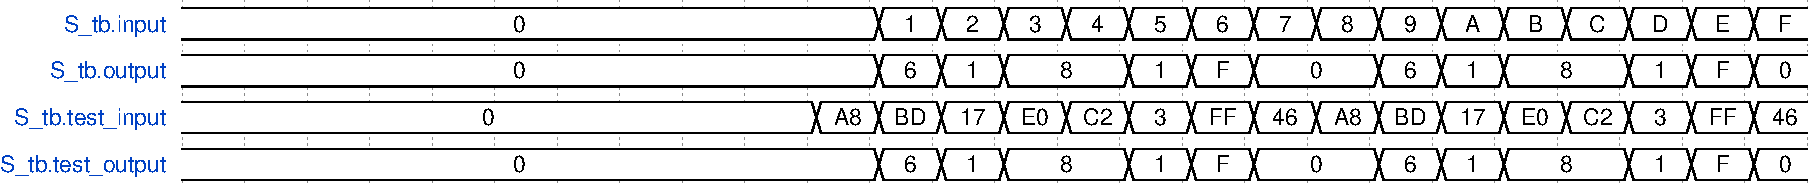
\includegraphics[width=\linewidth]{img/2_S_tb.pdf}
    \caption{Simulazione del sistema S}
    \label{fig:2_S_tb}
\end{figure}

\subsection{Esercizio 2.2}
In questo esercizio si passa all'implementazione su board dell'architettura vista nell'esercizio precedente.

\begin{code}
    \inputminted{vhdl}{vhdl/S_onboard.vhd}
    \caption{Implementazione del sistema S su board}
    \label{cod:S_onboard}
\end{code}

L'obiettivo è leggere un valore da un insieme di switch fisici e visualizzare il risultato su LED fisici. 

L'entity definisce i segnali di \texttt{input} e \texttt{output}:

\begin{itemize}
    \item \texttt{SW}: rappresentano l'ingresso del circuito, ovvero i bit dell'indirizzo usato per interrogare la ROM.
    \item \texttt{LED}: rappresentano l'uscita del circuito, ovvero il risultato elaborato dal modulo \texttt{S}, che viene mostrato visivamente.
\end{itemize}

L'uso degli switch e dei LED nei bit da 15 a 12 suggerisce che il codice è stato scritto per una scheda FPGA che ha un bus di I/O a 16 bit, ma per questo design si utilizzano solo i 4 bit più significativi.

L'architettura, che è \texttt{structural} [Codice sorgente \ref{cod:S_onboard}], è la parte in cui viene definito il comportamento interno. Viene dichiarato il modulo \texttt{S}, che riceve 4 bit in ingresso e restituisce 4 bit in uscita.

Infine, avviene il port mapping:

\begin{itemize}
    \item I 4 bit degli switch (\texttt{SW}) vengono collegati direttamente all'ingresso del modulo S.
    \item L'uscita del modulo \texttt{S} viene direttamente connessa ai 4 LED (\texttt{LED}).
\end{itemize}

Quindi, in linea di massima:

\begin{enumerate}
    \item L'utente imposta i 4 switch di sinistra su una combinazione binaria.
    \item Questo valore viene passato come indirizzo al modulo \texttt{S}, che legge il valore corrispondente dalla \texttt{ROM}.
    \item Il modulo \texttt{S} elabora il dato e restituisce un'uscita di 4 bit.
    \item L'uscita viene mostrata sui \texttt{LED}, che si accenderanno o spegneranno in base ai bit ricevuti.
\end{enumerate}

Per poter utilizzare la board è stato necessario effettuare alcune modifiche al file dei constraints \texttt{Nexys A7--100T--Master.xdc}. In particolare, abbiamo dovuto aggiungere i seguenti vincoli:
\begin{itemize}
    \item Abilitare gli switch \texttt{SW15}--\texttt{SW12} per l’input.
    \item Abilitare i LED \texttt{LED15}--\texttt{LED12} per la visualizzazione dell’output.
\end{itemize}
